\documentclass[12pt]{article}
\usepackage{multirow}
\usepackage[utf8x]{inputenc}
\usepackage[es-noshorthands]{babel} % Evitar interferencias de babel
\usepackage{amssymb,amsmath,amsthm,amsfonts}
\usepackage{mathrsfs}
\usepackage{calc}
\usepackage{graphicx}
\usepackage{subfigure}
\usepackage{gensymb}
\usepackage{threeparttable} %
\usepackage{url}
\usepackage{parskip}
\usepackage{fancyhdr}
\usepackage{float} 
\usepackage{vmargin}
\usepackage[style=apa, giveninits=true, isbn=false, maxbibnames=99, sorting=nyt]{biblatex} % Ya estás usando biblatex
\addbibresource{bibliografia.bib} % Aquí carga tu archivo .bib
\usepackage{setspace}
\usepackage{adjustbox}

% Paquete para hipervínculos
\usepackage{hyperref}
\hypersetup{
    colorlinks=true, % Colorear los hipervínculos
    linkcolor=black,  % Color de enlaces internos (citas)
    citecolor=black,  % Color de las citas
    filecolor=magenta,      
    urlcolor=cyan
}

\title{Proyecto Final}	
\date{04 de diciembre de 2024}						% Fecha

\makeatletter
\let\thetitle\@title
\let\theauthor\@author
\let\thedate\@date
\makeatother
\setlength{\parindent}{20pt}

\pagestyle{fancy}
\fancyhf{}
\cfoot{\thepage}

% Definición de estudiantes
\newcommand{\EstudianteUno}{José Carlos Quintero Cedeño C26152}
\newcommand{\EstudianteDos}{Joseph Romero Chinchilla C37006}
\newcommand{\EstudianteTres}{Diego Alberto Vega Víquez C38367}
\newcommand{\EstudianteCuatro}{Sofía Sequeira Ugalde B97458}

%%%%%%%%%%%%%%%%%%%%%%%%%%%%%%%%%%%%%%%%%%%%%%%%%%%%%%%%%%%%%%%%%%%%%
% Formateo de secciones e indice            									  
%%%%%%%%%%%%%%%%%%%%%%%%%%%%%%%%%%%%%%%%%%%%%%%%%%%%%%%%%%%%%%%%%%%%%
\usepackage{titlesec}
% Configuración para que las secciones no tengan número, pero aparezcan en el índice
\titleformat{\section}[block]{\normalfont\Large\bfseries}{\thesection}{1em}{}
\titlespacing*{\section}{0pt}{\baselineskip}{\baselineskip}
\titleformat{\subsection}[block]{\normalfont\large\bfseries}{\thesubsection}{1em}{}
\titlespacing*{\subsection}{0pt}{\baselineskip}{\baselineskip}
\titleformat{\subsubsection}[block]{\normalfont\normalsize\bfseries}{\thesubsubsection}{1em}{}
\titlespacing*{\subsubsection}{0pt}{\baselineskip}{\baselineskip}

% Comando para que las secciones sin número aparezcan en el índice
\setcounter{secnumdepth}{0}

%%%%%%%%%%%%%%%%%%%%%%%%%%%%%%%%%%%%%%%%%%%%%%%%%%%%%%%%%%%%%%%%%%%%%%%%%%%%%%%%%%%%%%%%%
\usepackage{multicol}

\providecommand{\comillas}[1]{``#1''} % Para escribir "a" entre comillas
\newcommand{\prts}[1]{\left( #1 \right)} % Para escribir "a" entre paréntesis
\newcommand{\corch}[1]{\left\{#1\right\}} % Para escribir "a" entre corchetes
\newcommand{\cuad}[1]{\left[#1\right]} % Para escribir "a" entre corchetes cuadrados
\newcommand{\abs}[1]{\lvert#1\rvert} % Para escribir el valor absoluto de "a"
\newcommand{\Abs}[1]{\begin{vmatrix} #1 \end{vmatrix}} % Para escribir el valor absoluto de "a" más grande
\newcommand{\intnom}[2]{{#1}^{(#2)}}
\newcommand{\var}[1]{\text{Var}\left[#1\right]} % es el simbolo de varianza
\newcommand{\E}[1]{\mathbb{E} \left[#1\right]} % Signo Esperanza
\renewcommand{\P}[1]{\mathbb{P} \left[#1\right]} % Signo Probabilidad

\usepackage{booktabs}
\usepackage{longtable}
\usepackage{hyperref}
\usepackage{siunitx}
\usepackage{lifecon}
\sisetup{
  group-separator={,},          % Coma como separador de miles
  group-minimum-digits=4,       % Activar separador de miles a partir de 4 dígitos
  round-mode=places,            % Redondeo por número de decimales
  round-precision=2,            % Precisamente dos decimales
  output-decimal-marker={.},    % Forzar el punto como separador decimal
  parse-numbers=false           % No intentar procesar el símbolo ₡
}

%%%%%%%%%%%%%%%%%%%%%%%%%%%%%%%%%%%%%%%%%%%%%%%%%%%%%%%%%%%%%%%%%%%%%%%%%%%%%%%%%%%%%%%%%

\begin{document}

%%%%%%%%%%%%%%%%%%%%%%%%%%%%%%%%%%%%%%%%%%%%%%%%%%%%%%%%%%%%%%%%%%%%%%%%%%%%%%%%%%%%%%%%%

\begin{titlepage}
	\centering
    \vspace*{0.0 cm}
    
    \textsc{\LARGE Universidad de Costa Rica}\\[1.0 cm]	% Nombre Universidad
	\textsc{\Large Teoría del interés}\\[0.5 cm]				% 
	\rule{\linewidth}{0.2 mm} \\[0.4 cm]

    % Establecer espaciado de 1.5 para el título
    \begin{spacing}{1.5}
        {\huge \bfseries \thetitle}\\
    \end{spacing}

	\rule{\linewidth}{0.2 mm} \\[1.5 cm]

    \vfill
    \begin{center}
      \large Estudiantes:%
      \linebreak %
      \linebreak %
      \begin{tabular}{c}
        \large \EstudianteUno  \\ \\
        \large \EstudianteDos  \\ \\
        \large \EstudianteTres  \\ \\
        \large \EstudianteCuatro 
      \end{tabular}
    \end{center}

    \vfill
	{\Large II Ciclo} \\[0.5 cm]
	{\large \thedate}\\[2 cm]
 
	\vfill
	
\end{titlepage}

%%%%%%%%%%%%%%%%%%%%%%%%%%%%%%%%%%%%%%%%%%%%%%%%%%%%%%%%%%%%%%%%%%%%%%%%%%%%%%%%%%%%%%%%%


% Redefinir el título de la tabla de contenidos
\renewcommand{\contentsname}{\centering \textbf{Tabla de Contenidos}}

\thispagestyle{empty}
\rule{\linewidth}{0.2 mm} 
\tableofcontents % Tabla de contenidos

\pagebreak


%%%%%%%%%%%%%%%%%%%%%%%%%%%%%%%%%%%%%%%%%%%%%%%%%%%%%%%%%%%%%%%%%%%%%%%%%%%%%%%%%%%%%%%%%

\setcounter{page}{1}

% punto (.) separador de decimales, coma (,) separador de miles.

\section{Introducción}

El presente informe tiene como objetivo asesorar a la empresa ABC en la toma de decisiones financieras estratégicas, abordando tres áreas críticas para su gestión: opciones de financiamiento, cobertura ante riesgos cambiarios y análisis del portafolio de inversión. Considerando el contexto actual con fecha de corte al 31 de octubre de 2024, se presentan análisis detallados y recomendaciones que buscan maximizar la rentabilidad y minimizar los riesgos financieros, alineándose con los objetivos de la empresa.

En primer lugar, se examinan las opciones de financiamiento para proyectos a cinco años, comparando los costos y flujos asociados a un crédito bancario y una emisión de bonos cuponados. Posteriormente, se aborda la gestión del riesgo cambiario mediante el uso de un contrato forward, incluyendo el cálculo del precio del contrato y proyecciones del tipo de cambio a mediano plazo. Por último, se realiza un análisis del portafolio de inversión, calculando métricas fundamentales como duración, duración modificada y convexidad, y proponiendo estrategias de inmunización para cumplir con obligaciones futuras a través de la compra o emisión de bonos.

Este informe se fundamenta en principios financieros sólidos, garantizando que las recomendaciones presentadas sean confiables y estén alineadas con las necesidades estratégicas de la empresa. Su objetivo es proporcionar a la empresa ABC una base clara y estructurada para tomar decisiones informadasque fortalezcan su posición financiera.


\newpage
\section{Sección I: Opciones de financiamiento}

La empresa ABC tiene proyectado realizar una inversión de 100 millones de colones en los próximos cinco años para llevar a cabo los diversos proyectos planificados. Con el objetivo de determinar la opción de financiamiento más adecuada, se presentan dos alternativas: una es la solicitud de un crédito en el Banco Credit Solutions (BCS) y la otra es la emisión de bonos cuponados en el mercado financiero. En esta sección se evaluarán ambas opciones para tomar una decisión informada.

\subsection{Crédito en el Banco Credit Solutions}

\textbf{Consideraciones iniciales}

El Banco Credit Solutions (BCS) ofrece 100 millones de colones con las siguientes condiciones:

\begin{itemize}
    \item Denotaremos $\intnom{i}{2}$ a la tasa de interés nominal convertible semestralmente. Para este caso $\intnom{i}{2} = 14 \%$, 
    \item El pago de los intereses se realizará al final de cada semestre. Esto quiere decir que se trabajará con anualidades inmediatas con $i = \intnom{i}{2}/2$. El interés efectivo semestral lo denotaremos $i$.
    \item La liquidación del crédito se hará mediante un pago único al final del período de cinco años (\textit{one lump-sum payment}).
    \item Para la amortización, se utilizará un fondo de amortización (\textit{sinking fund}), en el que la empresa realizará depósitos al final de cada trimestre durante los cinco años, con una tasa de interés anual efectiva de 7.5\%.
\end{itemize}

%Dado que se tiene la tasa de interés anual efectiva de 7.5\% para el fondo de amortización y los depósitos al mismo fondo se realizarán trimestralmente, conviene saber la tasa de interés efectiva que se acumula cada trimestre, esta corresponde a $i_{trim}$ la cual se calcula de la siguiente forma:

Dado que los depósitos al fondo de amortización se realizarán trimestralmente y la tasa de interés anual efectiva es de 7.5\%, se requiere calcular la tasa de interés efectiva trimestral, denotada como $i_{trim}$, utilizando la siguiente fórmula:

    \begin{equation}
        (1+i_{trim})^4 = (1+7.5\%) \implies i_{trim} = \sqrt[4]{1.075} -1 
        \label{interes.trimestral}
    \end{equation}
    
En esta sección se definirá lo siguiente:

    \begin{itemize}
        \item $K\cdot S_{\lcroof{n}\;i}$ representa el valor futuro de un pago de $K$ unidades monetarias al final de $n$ periodos a una tasa de interés $i$ .
        \item $K \cdot \prts{\dfrac{S_{\lcroof{n}\;i}}{S_{\lcroof{m}\;i}}}$ se refiere al valor futuro de un pago de $K$ unidades monetarias con $m$ periodos de conversión  de la tasa de interés en cada período de pago. $n$ es el número total de períodos de conversión, e $i$ es la tasa de interés por cada período de conversión.
        \item $X$ es la cantidad de dinero que la empresa ABC debe destinar trimestralmente para cubrir el crédito otorgado por el Banco Credit Solutions.
    \end{itemize}

\textbf{Desarrollo}

La ecuación para determinar el valor de $X$, que corresponde a la cantidad (en millones de colones) que debe destinarse trimestralmente, es la siguiente:

\begin{equation}
    X\cdot S_{\lcroof{20}\;i=i_{trim}} - 7 \cdot \prts{\dfrac{S_{\lcroof{20}\;i_{trim}}}{S_{\lcroof{2}\;i_{trim}}}} = 100
    \label{ecuación.principal}
\end{equation}        

Esta ecuación refleja que el valor futuro de los pagos trimestrales de $X$ millones al final de los 20 trimestres (5 años) menos el valor futuro de los pagos de 7 millones, realizados al final de cada dos trimestres (semestralmente), debe ser igual a 100 millones requeridos para liquidar el crédito mediante un pago único al final de los 5 años.

\textbf{Desglose de la ecuación}

%    \begin{itemize}
%        \item Primera parte:\\
%        \begin{center}
%            $X\cdot S_{\lcroof{20}\;i=i_{trim}}$
%        \end{center}
%        Representa los abonos que la empresa realiza trimestralmente a la cuenta de amortización. Aquí, $S_{\lcroof{20}\;i=i_{trim}}$ el factor de acumulación (valor futuro) para 20 trimestres, capitalizado trimestralmente al tipo de interés efectivo trimestral.
%        \item Segunda parte:\\
%        \begin{center}
%            $7 \cdot \prts{\frac{S_{\lcroof{20}\;i_{trim}}}{S_{\lcroof{2}\;i_{trim}}}}$
%        \end{center}
%        Representa los pagos de 7 millones realizados al final de cada dos trimestres (semestralmente). Aquí, se utiliza el cociente entre los factores de acumulación: $S_{\lcroof{20}\;i_{trim}}$ y $S_{\lcroof{2}\;i_{trim}}$ para 2 trimestres. Este cociente ajusta los valores al horizonte de 20 trimestres.
%    \end{itemize}

El término $X\cdot S_{\lcroof{20}\;i=i_{trim}}$ representa los abonos trimestrales realizados por la empresa al fondo de amortización, cuyo valor futuro se acumula durante 20 trimestres.

El término $7 \cdot \prts{\frac{S_{\lcroof{20}\;i_{trim}}}{S_{\lcroof{2}\;i_{trim}}}}$ refleja los pagos semestrales de 7 millones de colones. Aquí, se utiliza el cociente entre los factores de acumulación: $S_{\lcroof{20}\;i_{trim}}$ y $S_{\lcroof{2}\;i_{trim}}$ para 2 trimestres. Este cociente ajusta los valores al horizonte de 20 trimestres.

%\textbf{Interpretación de la ecuación}

La ecuación \eqref{ecuación.principal} se interpreta en el lado izquierdo las entradas y salidas de la cuenta de amortización:
    \begin{itemize}
        \item Entradas: Los pagos trimestrales de $X$, cuyo valor futuro se acumula al final del período de 20 trimestres.
        \item Salidas: Los pagos de 7 millones realizados semestralmente, ajustados para el mismo horizonte temporal (20 trimestres).
    \end{itemize}
    El lado derecho de la ecuación, igualado a 100, corresponde al monto total requerido al final del período para liquidar la deuda del crédito inicial.
    
\textbf{Solución de la ecuación}

Usando la definición del factor de acumulación para una anualidad inmediata de $n$ periodos a una tasa efectiva $i$ por periodo:

    \begin{equation}
        S_{\lcroof{n}\;i} = \dfrac{(1+i)^n-1}{i}
        \label{Definicion.FactorAcumulación}
    \end{equation}

A hora bien aplicando explícitamente \eqref{interes.trimestral} y \eqref{Definicion.FactorAcumulación} a la ecuación \eqref{ecuación.principal}, la ecuación queda de la siguiente forma:

\begin{center}
\small
    $X\cdot \prts{\dfrac{(1+(\sqrt[4]{1.075} -1))^{20}-1}{(\sqrt[4]{1.075} -1)}} - 7 \cdot \prts{\dfrac{\cuad{(1+(\sqrt[4]{1.075} -1))^{20}-1}/(\sqrt[4]{1.075} -1)}{\cuad{(1+(\sqrt[4]{1.075} -1))^{2}-1}/(\sqrt[4]{1.075} -1)}} = 100 $
\end{center}
    
Al realizar algunos cálculos, es sencillo observar que
    
    \begin{center}
        $X = \dfrac{100\prts{\sqrt[4]{1.075} -1}}{\prts{\sqrt[4]{1.075}}^{20}-1} + \dfrac{7\prts{\sqrt[4]{1.075} -1}}{\prts{\sqrt[4]{1.075}}^{2}-1} \approx 7.65646270$
    \end{center}

De esta forma se puede concluir que la cuota mensual que debe destinarse cada trimestre corresponde a ₡{7,656,462.70}.% 7656462.70480034

\textbf{Adicional}

Este cálculo también podría haberse resuelto utilizando ecuaciones en diferencias. En particular, sería necesario resolver el caso general de la siguiente ecuación:

\begin{center}
    $S_n = (1+i_{trim})\cdot S_{n-1} + \left(X - \frac{1+(-1)^n}{2} \cdot 7 \right)$
\end{center}
        
Con la condición inicial \( S_0 = 0 \). En esta ecuación, \( S_n \) representa el saldo de la cuenta de amortización al final del \( n \)-ésimo trimestre. Una vez resuelta la ecuación y obtenido un criterio para \( S_n \) que dependa únicamente de \( n \), basta con evaluar la solución en \( n=20 \) e igualarla a 100.

La solución general a esta ecuación es:
        
\begin{center}
    $S_n = \displaystyle\sum_{r=1}^n \left(X - \frac{1+(-1)^r}{2} \cdot 7 \right)(1+i_{trim})^{n-r}$
\end{center}
        
De esta forma, si consideramos la ecuación \eqref{interes.trimestral}, planteamos \( S_{20} = 100 \) y resolvemos para \( X \). Este procedimiento produce el mismo resultado que el obtenido previamente. Este enfoque se menciona porque fue el método utilizado para derivar la ecuación \eqref{ecuación.principal}.

\subsubsection{Tabla de Amortización}

El Cuadro \ref{tabla1b} detalla los flujos financieros de la cuenta de amortización diseñados para liquidar una deuda mediante un pago único al final de un periodo de 20 trimestres. Este instrumento permite visualizar la evolución del saldo en la cuenta, considerando tanto los depósitos trimestrales como los intereses generados para cumplir con las obligaciones intermedias.

Es importante mencionar que en los meses impares se paga la totalidad dispuesta para ese trimestre $X=₡7,656,462.70$ y en los impares se paga $X$ menos los intereses que se le deben pagar a BCS. Además cabe destacar que se asume que los depósitos se empiezan a realizar a finales de enero del siguiente año (31/01/2025). Este esquema permite a la empresa ABC garantizar que el fondo acumulado sea suficiente para realizar el pago único (\textit{one lump-sum payment}) al final del plazo. Además, destaca la eficiencia del mecanismo de capitalización de intereses, que contribuye significativamente al crecimiento del saldo acumulado.

\setlength{\abovecaptionskip}{10pt} % Aj
\begin{table}[H]
\centering
\caption{Tabla de Amortización Trimestral en Colones}
\begin{adjustbox}{max width=\textwidth}
\begin{threeparttable}
\vspace{0.1cm}
\begin{tabular}{llrrrrr}
\hline\hline
        \textbf{Fecha} & \textbf{Periodo} & \textbf{Int. Pagado} & \textbf{Depósitos} & \textbf{Int. Fondo} & \textbf{Saldo} & \textbf{Amortización} \\ \hline
              31/10/2024 & Trimestre 0 & 0.00 & 0.00 & 0.00 & 0.00 & 100,000,000.00 \\ 
              31/01/2025 & Trimestre 1 & 0.00 & 7,656,462.70 & 0.00 & 7,656,462.70 & 92,343,537.30 \\ 
              01/05/2025 & Trimestre 2 & 7,000,000.00 & 656,462.70 & 139,689.11 & 8,452,614.52 & 91,547,385.48 \\ 
              31/07/2025 & Trimestre 3 & 0.00 & 7,656,462.70 & 154,214.58 & 16,263,291.80 & 83,736,708.20 \\ 
              31/10/2025 & Trimestre 4 & 7,000,000.00 & 656,462.70 & 296,717.27 & 17,216,471.78 & 82,783,528.22 \\ 
              31/01/2026 & Trimestre 5 & 0.00 & 7,656,462.70 & 314,107.66 & 25,187,042.14 & 74,812,957.86 \\ 
              01/05/2026 & Trimestre 6 & 7,000,000.00 & 656,462.70 & 459,527.54 & 26,303,032.38 & 73,696,967.62 \\ 
              31/07/2026 & Trimestre 7 & 0.00 & 7,656,462.70 & 479,888.33 & 34,439,383.42 & 65,560,616.58 \\ 
              31/10/2026 & Trimestre 8 & 7,000,000.00 & 656,462.70 & 628,332.81 & 35,724,178.94 & 64,275,821.06 \\ 
              31/01/2027 & Trimestre 9 & 0.00 & 7,656,462.70 & 651,773.39 & 44,032,415.04 & 55,967,584.96 \\ 
              01/05/2027 & Trimestre 10 & 7,000,000.00 & 656,462.70 & 803,353.85 & 45,492,231.59 & 54,507,768.41 \\ 
              31/07/2027 & Trimestre 11 & 0.00 & 7,656,462.70 & 829,987.62 & 53,978,681.92 & 46,021,318.08 \\ 
              31/10/2027 & Trimestre 12 & 7,000,000.00 & 656,462.70 & 984,819.52 & 55,619,964.14 & 44,380,035.86 \\ 
              31/01/2028 & Trimestre 13 & 0.00 & 7,656,462.70 & 1,014,764.06 & 64,291,190.90 & 35,708,809.10 \\ 
              01/05/2028 & Trimestre 14 & 7,000,000.00 & 656,462.70 & 1,172,967.13 & 66,120,620.74 & 33,879,379.26 \\ 
              31/07/2028 & Trimestre 15 & 0.00 & 7,656,462.70 & 1,206,344.35 & 74,983,427.80 & 25,016,572.20 \\ 
              31/10/2028 & Trimestre 16 & 7,000,000.00 & 656,462.70 & 1,368,042.73 & 77,007,933.23 & 22,992,066.77 \\ 
              31/01/2029 & Trimestre 17 & 0.00 & 7,656,462.70 & 1,404,979.02 & 86,069,374.96 & 13,930,625.04 \\ 
              01/05/2029 & Trimestre 18 & 7,000,000.00 & 656,462.70 & 1,570,301.41 & 88,296,139.07 & 11,703,860.93 \\ 
              31/07/2029 & Trimestre 19 & 0.00 & 7,656,462.70 & 1,610,927.84 & 97,563,529.62 & 2,436,470.38 \\ 
              31/10/2029 & Trimestre 20 & 107,000,000.00 & 656,462.70 & 1,780,007.68 & 100,000,000.00 & 0.00 \\ \hline \hline     
\end{tabular}
 \begin{tablenotes}
	\item[] \small\textbf{Fuente:} Elaboración propia.
\end{tablenotes} 
\end{threeparttable}
\end{adjustbox}
\label{tabla1b}
 \end{table}


%mejorar esto hasta antes de la interpretacion de la tabla.
\subsection{Emisión de bonos cuponados} 

La empresa ABC puede emitir bonos cuponados con las siguientes condiciones:

\begin{itemize}
    \item Tasa facial de 3\%.
    \item Cupones con pago bimensual.
\end{itemize}

Dado que la tasa facial es de 3\%, el precio del bono es:

\[ 100,000,000 \cdot 0.03\% = 3,000,000 \] 

Para valorar los flujos en el año 2.5, se utiliza el precio del bono cero cupón ajustado por la Curva Bono Cero Cupón (CBCC) del Banco Central de Costa Rica (BCCR). Este precio representa el factor de descuento necesario para calcular el valor presente de un flujo en 2.5 años y se define como:

\[ P(0;2.5) = \frac{1}{(1.0535)^{2.5}} = 88\% \]

En el caso de los bonos cuponados, los flujos se ajustan considerando que la CBCC permite reflejar las condiciones del mercado en fechas específicas. Por lo tanto, el cálculo del valor equivalente en 2.5 años se realiza de la siguiente manera:

\[ 3,000,000 \cdot \frac{CBCC}{P(0;2.5)} \]

Donde la CBCC corresponde al valor ajustado de la curva en la fecha específica.

De manera similar, los flujos del crédito se ajustan utilizando el mismo procedimiento. 

\[ 7,000,000  \cdot \frac{CBCC}{P(0;2.5)} \]

De esta forma, se calculan los valores equivalentes en el año 2.5 para ambas alternativas de financiamiento.

En el Cuadro \ref{tabla1c}, se presentan los resultados de los flujos de efectivo correspondientes a cada alternativa de financiamiento. Podemos observar que el financiamiento por crédito tiene una estructura de pagos concentrada en períodos específicos con montos mayores, mientras que el financiamiento por bonos cuponados distribuye los pagos en montos más constantes a lo largo del tiempo. 

En términos del total acumulado, el financiamiento por crédito implica un desembolso total de ₡153,427,395, que resulta menor en comparación con el financiamiento por bonos cuponados, cuyo total asciende a ₡173,975,653. Esto sugiere que, desde una perspectiva de costo total, el crédito es más económico. Por lo tanto, se recomienda a la empresa ABC optar por la alternativa de financiamiento de crédito debido a su menor costo total.


\begin{table}[H]
\centering
\caption{Valor de los flujos de las alternativas de financiamiento en el año 2.5 en colones}
\begin{threeparttable}
\vspace{0.1cm}
\begin{tabular}{lrr}
\hline\hline
\textbf{Fecha} & \textbf{Crédito} & \textbf{Bonos cuponados} \\ \hline
31/12/2024 & 0 &  3,393,341 \\
28/02/2025 & 0 &  3,369,328 \\
30/04/2025 & 7,802,178 & 3,343,791 \\
30/06/2025 & 0 & 3,317,661 \\
31/08/2025 & 0 & 3,290,454 \\
31/10/2025 & 7,614,273 & 3,263,260 \\
31/12/2025 & 0 & 3,235,343 \\
28/02/2026 & 0 & 3,208,192 \\
30/04/2026 & 7,418,743 & 3,179,461 \\
30/06/2026 & 0 & 3,150,483 \\
31/08/2026 & 0 & 3,120,639 \\
31/10/2026 & 7,211,387 & 3,090,594 \\
31/12/2026 & 0 & 3,061,014 \\
28/02/2027 & 0 & 3,031,542 \\
30/04/2027 & 7,002,485 & 3,001,065 \\
30/06/2027 & 0 & 2,970,646 \\
31/08/2027 & 0 & 2,939,451 \\
31/10/2027 & 6,786,003 & 2,908,287 \\
31/12/2027 & 0 & 2,877,989 \\
28/02/2028 & 0 & 2,847,257 \\
30/04/2028 & 6,571,579 & 2,816,391 \\
30/06/2028 & 0 & 2,784,843 \\
31/08/2028 & 0 & 2,753,538 \\
31/10/2028 & 6,351,153 & 2,722,351 \\
31/12/2028 & 0 & 2,691,403 \\
28/02/2029 & 0 & 2,661,351 \\
30/04/2029 & 6,136,932 & 2,630,114 \\
30/06/2029 & 0 & 2,600,094 \\
31/08/2029 & 0 & 2,568,471 \\
31/10/2029 & 90,531,662 & 87,147,301 \\ \hline 
\textbf{Total} & 153,427,395 & 173,975,653 \\ \hline \hline 
\end{tabular}
 \begin{tablenotes}
	\item[] \small\textbf{Fuente:} Elaboración propia.
\end{tablenotes} 
\end{threeparttable}
\label{tabla1c}
 \end{table}

\newpage
\section{Sección II: Contrato forward de tipo de cambio}

%\section*{Análisis del Contrato Forward de Tipo de Cambio y Estrategia para Mitigación de Riesgo Cambiario}

\subsection{Determinación del precio del contrato forward}

Para determinar el precio en colones del contrato forward, es fundamental replicar los flujos futuros del contrato en el momento \( T \) mediante una estrategia de inversión equivalente. Este enfoque se basa en el principio de \textbf{ausencia de arbitraje}, que establece que dos activos con flujos de efectivo idénticos deben tener el mismo precio. De lo contrario, sería posible obtener ganancias sin riesgo mediante arbitraje al comprar el activo más barato y vender el más caro.

La estrategia para replicar los flujos del contrato forward es la siguiente:

\begin{enumerate}
    \item \textbf{Venta de bonos cero cupón en colones}: Se venden bonos cero cupón por un monto nominal de \( K \) colones en el momento \( t \). Esto garantiza que en el momento \( T \) se tendrá la obligación de pagar \( K \) colones.
    \item \textbf{Compra de un bono cero cupón en dólares}: Se adquiere un bono cero cupón de la Reserva Federal de Estados Unidos (FED) en el momento \( t \), con un valor de compra equivalente a \( E_t \cdot P_{\text{\$}}(t, T) \) colones, donde \( E_t \) es el tipo de cambio actual y \( P_{\text{\$}}(t, T) \) es el precio del bono. Este bono garantizará la entrega de 1 dólar en \( T \), que al venderse se convierte en \( E_T \) colones en ese momento.
\end{enumerate}

El costo de esta estrategia en \( t \) es:
\[ K \cdot P_{\text{₡}}(t, T) - E_t P_{\text{\$}}(t, T), \]

donde \( P_{\text{₡}}(t, T) \) representa el precio actual de un bono cero cupón en colones. Este valor corresponde al precio justo del contrato forward, ya que replica perfectamente los flujos futuros.

La tabla a continuación resume los flujos de esta estrategia:

\begin{table}[h!]
        \centering
        \caption{Flujos de la estrategia de inversión.}
        \begin{tabular}{ c c c | c}
        \hline
            \textbf{Tiempo} & \textbf{Se recibe} & \textbf{Se paga} & \textbf{Flujo Neto}\\  \hline 
            $t$ & {$K \cdot P_{\text{₡}}(t, T)$} & {$ E_t P_{\text{\$}}(t, T)$} & {$K \cdot P_{\text{₡}}(t, T) - E_t P_{\text{\$}}(t, T)$} \\
            $T$ & {$E_T$} & {$K$} & $E_T - K$ \\
            \hline \\
        \end{tabular}
        \begin{tablenotes}
	\item[] \small\textbf{Fuente:} Elaboración propia.
\end{tablenotes}
    \end{table}

\subsection{Proyección del tipo de cambio futuro}

 Para anticipar el comportamiento del tipo de cambio y calcular el forward, es necesario identificar el monto \( K \) que hace que el valor del contrato en \( t \) sea cero. Este valor se obtiene como:
\[ K = \frac{E_t \cdot P_{\text{\$}}(t, T)}{P_{\text{₡}}(t, T)}, \]
lo que indica el tipo de cambio forward.

Esta fórmula implica que el tipo de cambio forward es el mejor estimador del tipo de cambio esperado \( E_T \) bajo el principio de ausencia de arbitraje. La lógica detrás de esto es que, si ambas partes del contrato se ponen de acuerdo en que intercambiar \( E_T \) por $\frac{E_t \cdot P_{\text{\$}}(t, T)}{P_{\text{₡}}(t, T)}$ en \( T \) hace que el precio del contrato sea 0, entonces eso significa que a ambas partes les es indiferente participar o no en el contrato; en otras palabras, para la empresa ABC sería lo mismo asegurar un intercambio de \( E_T \) por $\frac{E_t \cdot P_{\text{\$}}(t, T)}{P_{\text{₡}}(t, T)}$ a través de un contrato forward de tipo de cambio o simplemente esperar a pagar el \( E_T \) que determine el mercado en el futuro. 

Por tanto, para la planificación presupuestaria de la empresa, el valor de $\frac{E_t \cdot P_{\text{\$}}(t, T)}{P_{\text{₡}}(t, T)}$ debe ser tomado como referencia para prever el costo de los insumos en dólares al final de cada mes durante los próximos cinco años. 

Seguidamente se muestra un gráfico que representa visualmente dicha proyección del tipo de cambio futuro.

\begin{figure}[H]
\renewcommand{\figurename}{Gráfico}
\caption{Proyección del tipo de cambio \( E_T \) en los próximos 5 años}
    \centering
    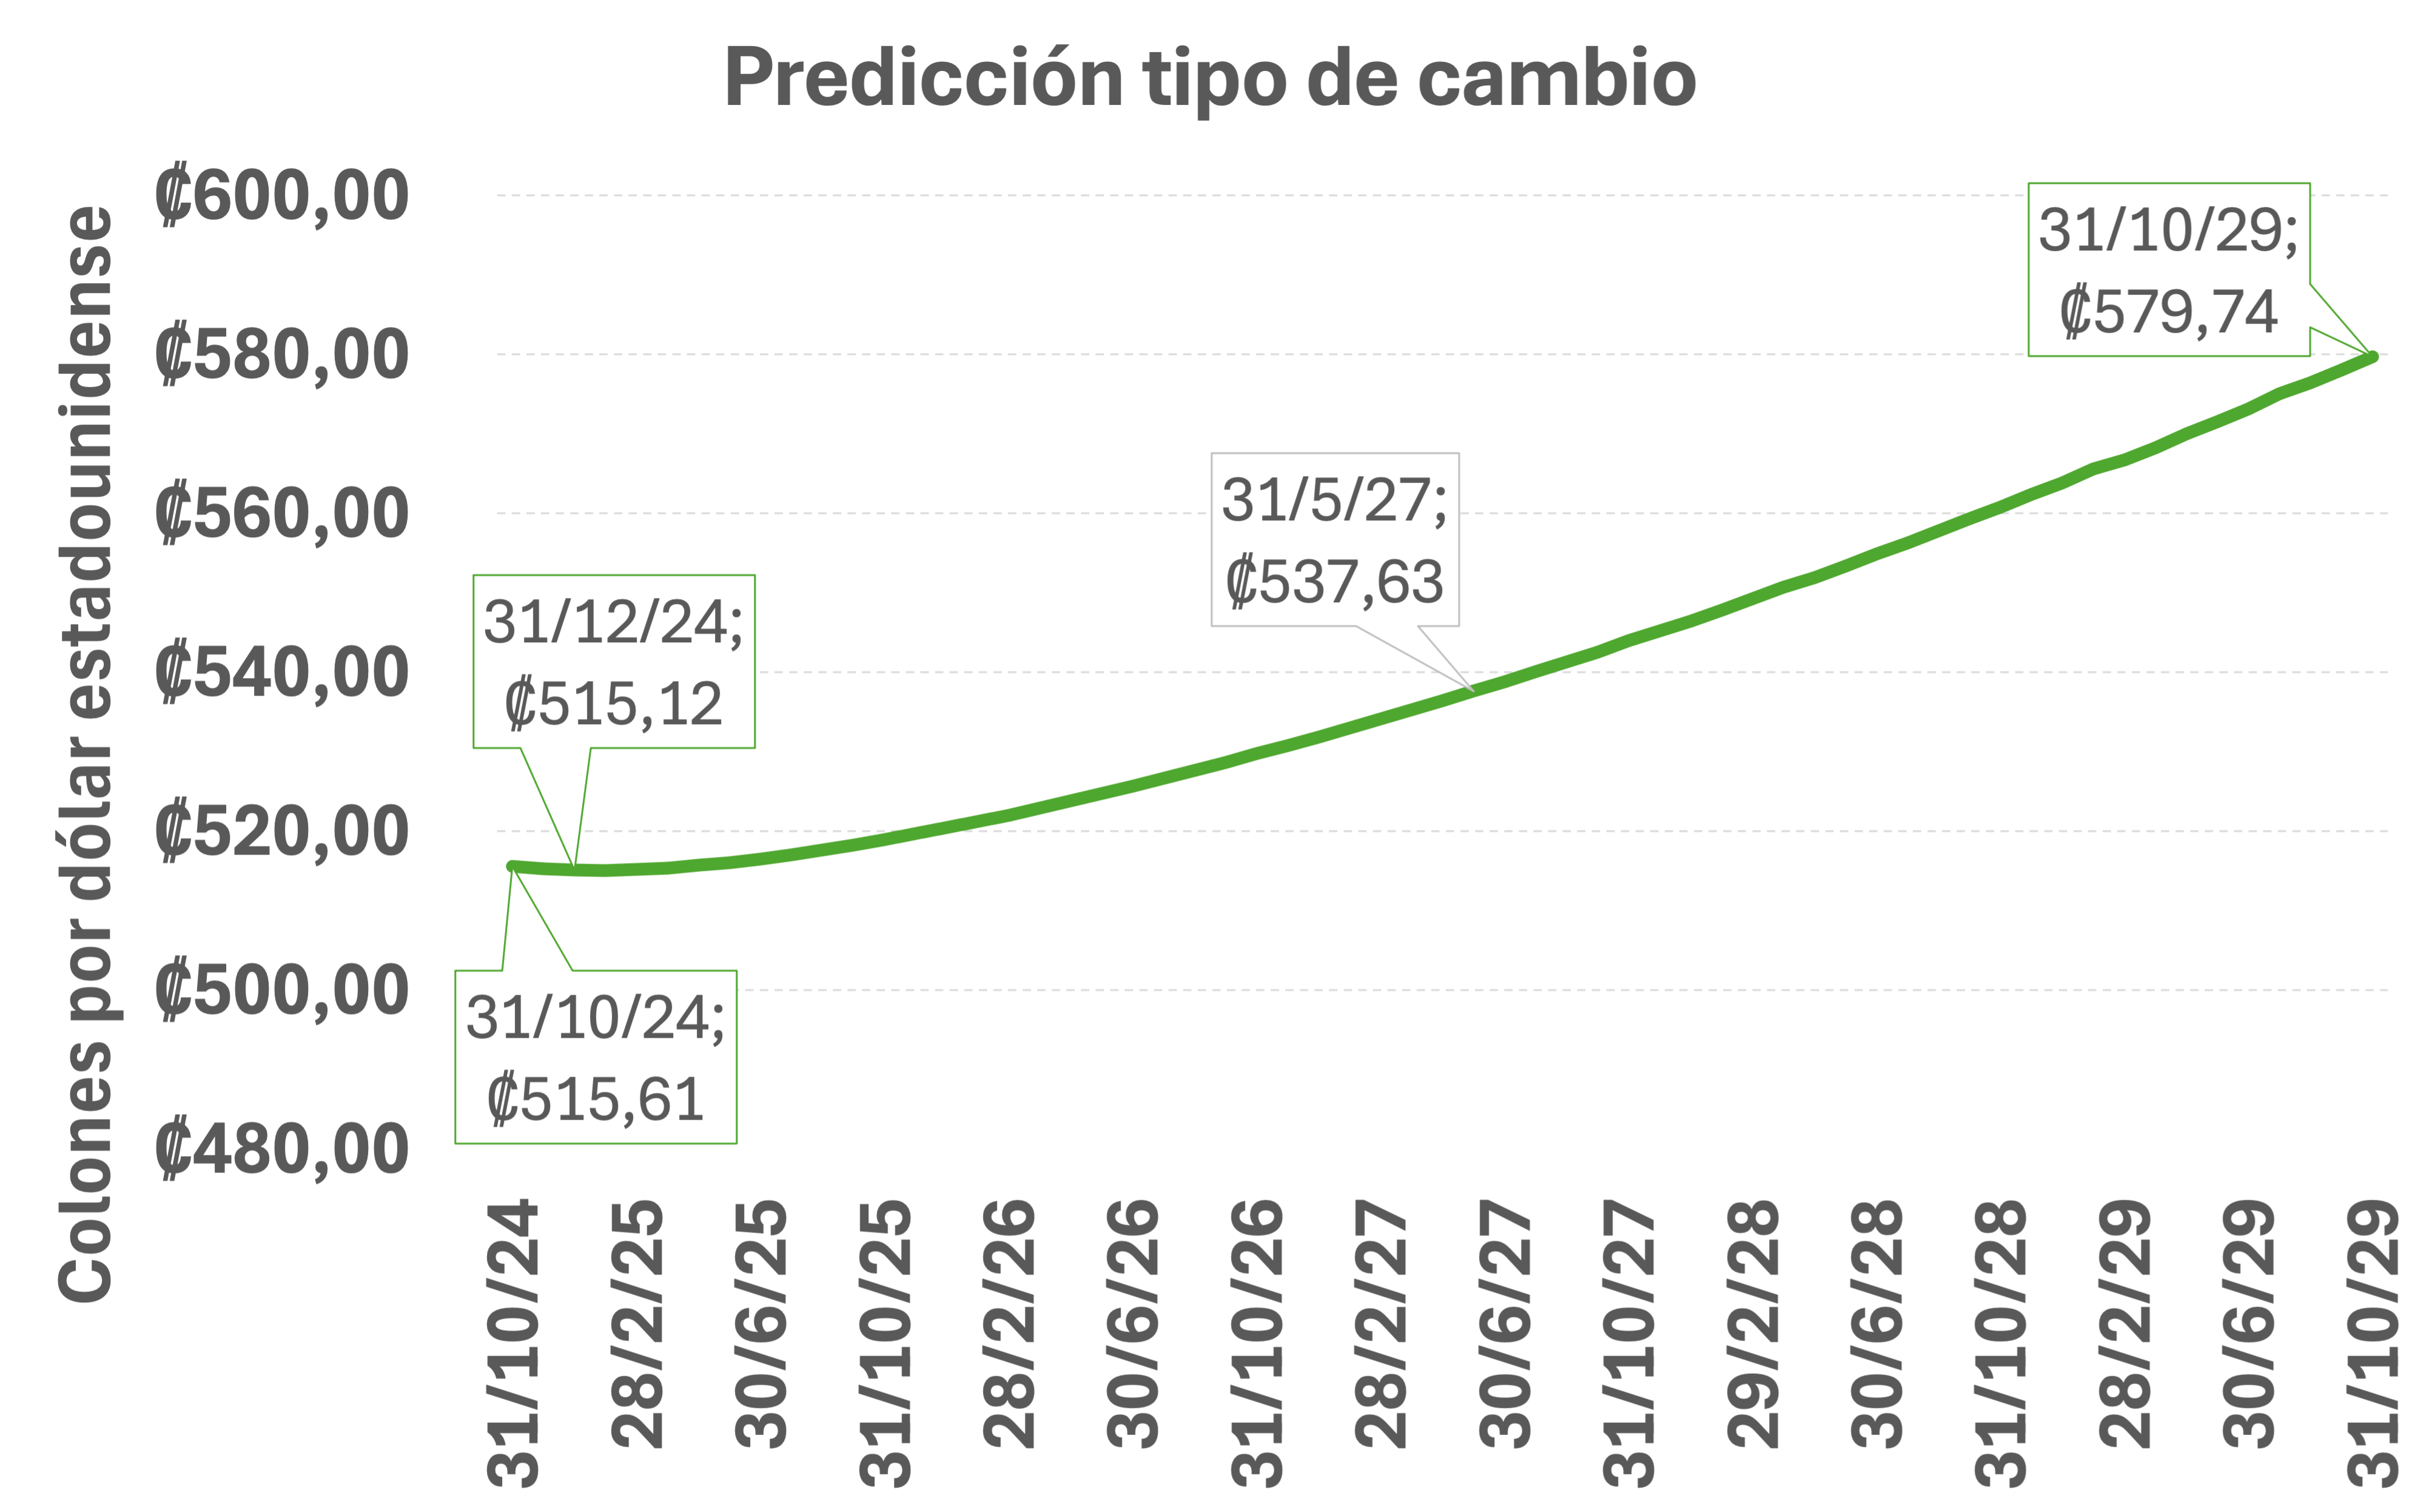
\includegraphics[width=0.9\textwidth]{grafico_tipo_de_cambio.png}
    \small\textbf{Fuente:} Elaboración propia.
    \label{fig:enter-label}
\end{figure}

En forma tabular, los datos corresponden a:


%\subsubsection{Predicción de Tipo de Cambio}

\newpage
\begin{table}[h!] % Ambiente para la tabla
\centering % Centrar el contenido
\caption{Predicción del tipo de cambio proyectado.}
\label{tab:prediccion_tipo_cambio} % Etiqueta para referencias
\begin{multicols}{2} % Divide el contenido en dos columnas
\noindent
\begin{tabular}{lr}
  \hline \hline
  Fecha & Predicción \\ 
  \hline
  31/10/2024 & ₡515.61 \\ 
  30/11/2024 & ₡515.28 \\ 
  31/12/2024 & ₡515.12 \\ 
  31/01/2025 & ₡515.11 \\ 
  28/02/2025 & ₡515.19 \\ 
  31/03/2025 & ₡515.40 \\ 
  30/04/2025 & ₡515.71 \\ 
  31/05/2025 & ₡516.06 \\ 
  30/06/2025 & ₡516.52 \\ 
  31/07/2025 & ₡517.08 \\ 
  31/08/2025 & ₡517.67 \\ 
  30/09/2025 & ₡518.26 \\ 
  31/10/2025 & ₡518.97 \\ 
  30/11/2025 & ₡519.69 \\ 
  31/12/2025 & ₡520.51 \\ 
  31/01/2026 & ₡521.27 \\ 
  28/02/2026 & ₡522.02 \\ 
  31/03/2026 & ₡522.94 \\ 
  30/04/2026 & ₡523.84 \\ 
  31/05/2026 & ₡524.77 \\ 
  30/06/2026 & ₡525.68 \\ 
  31/07/2026 & ₡526.66 \\ 
  31/08/2026 & ₡527.64 \\ 
  30/09/2026 & ₡528.68 \\ 
  31/10/2026 & ₡529.80 \\ 
  30/11/2026 & ₡530.78 \\ 
  31/12/2026 & ₡531.87 \\ 
  31/01/2027 & ₡533.00 \\ 
  28/02/2027 & ₡534.11 \\ 
  31/03/2027 & ₡535.33 \\
  \hline \hline
\end{tabular}

\columnbreak % Cambia a la segunda columna

\noindent
\begin{tabular}{lr}
  \hline \hline
  Fecha & Predicción \\ 
  \hline
  30/04/2027 & ₡536.42 \\ 
  31/05/2027 & ₡537.63 \\ 
  30/06/2027 & ₡538.78 \\ 
  31/07/2027 & ₡540.12 \\ 
  31/08/2027 & ₡541.31 \\ 
  30/09/2027 & ₡542.53 \\ 
  31/10/2027 & ₡543.98 \\ 
  30/11/2027 & ₡545.22 \\ 
  31/12/2027 & ₡546.43 \\ 
  31/01/2028 & ₡547.80 \\ 
  29/02/2028 & ₡549.23 \\ 
  31/03/2028 & ₡550.69 \\ 
  30/04/2028 & ₡551.95 \\ 
  31/05/2028 & ₡553.39 \\ 
  30/06/2028 & ₡554.87 \\ 
  31/07/2028 & ₡556.25 \\ 
  31/08/2028 & ₡557.78 \\ 
  30/09/2028 & ₡559.35 \\ 
  31/10/2028 & ₡560.80 \\ 
  30/11/2028 & ₡562.36 \\ 
  31/12/2028 & ₡563.86 \\ 
  31/01/2029 & ₡565.59 \\ 
  28/02/2029 & ₡566.73 \\ 
  31/03/2029 & ₡568.24 \\ 
  30/04/2029 & ₡570.00 \\ 
  31/05/2029 & ₡571.56 \\ 
  30/06/2029 & ₡573.13 \\ 
  31/07/2029 & ₡575.03 \\ 
  31/08/2029 & ₡576.41 \\ 
  30/09/2029 & ₡578.02 \\ 
  31/10/2029 & ₡579.74 \\ 
  \hline \hline
\end{tabular}
\end{multicols}
\begin{tablenotes}
	\item[] \small\textbf{Fuente:} Elaboración propia.
\end{tablenotes}
\end{table}

\subsection{Escenario de arbitraje: tipo de cambio futuro de ₡500 por dólar}

En el escenario hipotético donde el tipo de cambio efectivo al 31 de diciembre de 2024 sea \( E_T = 500 \, \text{colones/dólar} \), se observa que este valor sería menor al tipo de cambio forward calculado como:
\[ k = \frac{E_t \cdot P_{\$}(t, T)}{P_{\text{₡}}(t, T)} = 515.12 \]

Surgiría una oportunidad de arbitraje:

\begin{itemize}
    \item Un arbitrajista vende un contrato forward de tipo de cambio, comprometiéndose a entregar \( E_T \) colones a cambio de \( k \).
    \item En este caso, se asegura una ganancia igual a:
    \[ k - E_T = \frac{E_t \cdot P_{\text{\$}}(t, T)}{P_{\text{₡}}(t, T)} - 500 = 15.12 \] colones por dólar.
\end{itemize}

Dado que el contrato forward se negocia de forma que su precio inicial sea cero, no habría costos presentes, lo que garantiza que cualquier diferencia futura positiva entre \( k \) y \( E_T \) represente una ganancia asegurada para el arbitrajista.



\newpage
\section{Sección III: Portafolio de inversión}

Se debe tener en cuenta que el análisis considera el dinero recibido en el día de hoy.

\subsection{Índices financieros del portafolio}

El análisis de un portafolio de bonos requiere comprender su comportamiento frente a cambios en las tasas de interés. En este caso, se calculan tres índices clave: \textbf{duración}, \textbf{volatilidad} y \textbf{convexidad}. Estos índices permiten evaluar la sensibilidad del portafolio a las tasas de interés, lo que es esencial para gestionar el riesgo y tomar decisiones informadas sobre ajustes en la cartera.

\subsubsection{Datos del Portafolio}

El portafolio de la empresa ABC está compuesto por una combinación de bonos cero cupón y bonos cuponados, con diferentes características en términos de tasa de cupón, vencimiento y periodicidad de pago. Los datos de los bonos son los siguientes:

\begin{table}[H]
\centering
\small
\caption{Bonos del Portafolio} 
\vspace{0.1cm} 
\begin{tabular}{lcccc}
\hline \hline
\textbf{Tipo} & \textbf{Valor Facial} & \textbf{Tasa de Cupón} & \textbf{Vencimiento} & \textbf{Periodicidad} \\ 
 & \textbf{(₡)} &  &  & \textbf{(meses)} \\ 
\midrule
Cero Cupón & 10,000,000  & 0     & 2025-03-18 & N/A  \\
Cero Cupón & 35,000,000  & 0     & 2028-10-31 & N/A  \\
Cero Cupón & 80,000,000  & 0     & 2029-08-15 & N/A  \\
Cuponado   & 15,000,000  & 0.03  & 2026-01-31 & 4    \\
Cuponado   & 20,000,000  & 0.02  & 2027-02-28 & 12   \\
Cuponado   & 23,000,000  & 0.04  & 2029-06-30 & 3    \\
Cuponado   & 40,000,000  & 0.07  & 2030-04-30 & 2    \\
\hline \hline
\end{tabular}
\begin{tablenotes}
	\item[] \small\textbf{Fuente:} Elaboración propia.
\end{tablenotes}
\end{table}

\subsubsection{Cálculo de Índices Financieros}

El análisis de los índices financieros se basa en tres conceptos clave: \textbf{duración}, \textbf{volatilidad} y \textbf{convexidad}, que se calculan con base en los flujos de efectivo de los bonos y las tasas de interés asociadas.

\noindent \textbf{Duración}

La duración es una medida que cuantifica el tiempo promedio ponderado hasta que se recuperan los flujos de efectivo de un bono. Este índice es crucial para entender cómo un bono o un portafolio de bonos reacciona a cambios en las tasas de interés. Una duración más larga significa que el bono o portafolio será más sensible a las variaciones en las tasas.

La fórmula para la duración de un bono es:

\[
D^{(i)} = \frac{\sum_{t=1}^n \tau(t, T_t) \cdot CF_t \cdot (1 + \rho(t, T_t))^{-\tau(t, T_t)}}{\sum_{t=1}^n CF_t \cdot (1 + \rho(t, T_t))^{-\tau(t, T_t)}},
\]

donde:
\begin{itemize}
    \item \( \tau(t, T_t) = \frac{\text{Días entre } t \text{ y } T_t}{365.25} \) es el tiempo hasta el vencimiento expresado en años,
    \item \( CF_t \) es el flujo de efectivo en el tiempo \( t \),
    \item \( \rho(t, T_t) \) es la tasa de interés para el vencimiento \( T_t \) en el tiempo \( t \).
\end{itemize}

Para el portafolio de bonos, la duración del portafolio \( D \) se calcula como la duración ponderada de cada bono, ajustada por el porcentaje que cada bono representa en el valor total del portafolio:

\[
D = \frac{P^{(1)} \cdot D^{(1)}}{P} + \frac{P^{(2)} \cdot D^{(2)}}{P} + \cdots + \frac{P^{(m)} \cdot D^{(m)}}{P},
\]

donde:
\begin{itemize}
    \item \( P^{(i)} \) es el precio del bono \( i \),
    \item \( D^{(i)} \) es la duración del bono \( i \),
    \item \( P \) es el valor total del portafolio, dado por \( P = P^{(1)} + P^{(2)} + \cdots + P^{(m)} \).
\end{itemize}

Expandiendo la fórmula de duración del portafolio con la definición de \( D^{(i)} \), obtenemos:

\[
D = \frac{P^{(1)} \cdot \frac{\sum_{t=1}^n \tau(t, T) \cdot CF_t^{(1)} \cdot (1 + \rho(t, T))^{-\tau(t, T)}}{P^{(1)}}}{P} + \cdots + \frac{P^{(m)} \cdot \frac{\sum_{t=1}^n \tau(t, T) \cdot CF_t^{(m)} \cdot (1 + \rho(t, T))^{-\tau(t, T)}}{P^{(m)}}}{P}.
\]

Simplificando, se puede escribir como:

\[
D = \frac{\sum_{t=1}^n \tau(t, T) \cdot \big(CF_t^{(1)} + \cdots + CF_t^{(m)}\big) \cdot (1 + \rho(t, T))^{-\tau(t, T)}}{P}.
\]

En esta expresión:
\begin{itemize}
    \item La suma de los flujos de efectivo ponderados por \( \tau(t, T) \) y descontados por \( (1 + \rho(t, T))^{-\tau(t, T)} \) representa la contribución de todos los bonos en el portafolio.
    \item El denominador \( P \) normaliza esta contribución al valor total del portafolio.
\end{itemize}

Por lo tanto, la duración del portafolio es el promedio ponderado de las duraciones de sus componentes. Esto refleja cómo los cambios en la tasa de interés afectan el valor total del portafolio, tomando en cuenta tanto las características individuales de los bonos como su relevancia dentro del portafolio.

\noindent \textbf{Volatilidad}

La volatilidad mide cómo un bono o portafolio de bonos reacciona a los cambios en las tasas de interés. Específicamente, se trata de la sensibilidad del precio del bono ante cambios en las tasas. Un bono con alta volatilidad tendrá un precio más sensible a las fluctuaciones de las tasas de interés.

La fórmula para calcular la volatilidad de un bono es la siguiente:
\[
V = \sum_{t=1}^n \tau(t, T) \cdot CF_t \cdot (1 + \rho(t, T))^{-(\tau(t, T)+1)},
\]
donde \(T\) representa el vencimiento del bono y \(CF_t\) los flujos de efectivo en cada periodo.


De manera similar a la duración, la volatilidad total de un portafolio se obtiene ponderando la volatilidad de cada bono según su proporción dentro del valor total del portafolio. Esto permite una evaluación más precisa del riesgo asociado a la variabilidad de los precios en un conjunto de bonos. La volatilidad proporciona una medida proporcional de cómo varía el precio de un bono por un cambio unitario en la tasa de interés. Por ejemplo, si la volatilidad es \( V = 0.05 \), esto indica que un incremento del 1\% en la tasa de interés resultará en una caída aproximada del 5\% en el precio del bono, y viceversa. Para un portafolio de bonos, la \textbf{volatilidad del portafolio} se calcula como el promedio ponderado de la volatilidad de sus componentes.


\noindent \textbf{Convexidad}

La convexidad mide la curvatura de la relación entre el precio de un bono y las tasas de interés. Mientras que la duración evalúa la sensibilidad lineal del precio ante pequeños cambios en las tasas de interés, la convexidad se encarga de capturar los efectos no lineales. En otras palabras, permite medir cómo cambia la sensibilidad del precio (duración) ante variaciones más grandes en las tasas de interés.

Un bono con una convexidad más alta tiende a ser más estable frente a grandes fluctuaciones en las tasas, ya que su precio reacciona de manera más moderada. Por esta razón, la convexidad es particularmente útil para gestionar el riesgo de interés en entornos de alta volatilidad.

La fórmula para la convexidad de un bono es:

\[
C = \frac{1}{P} \sum_{t=1}^n CF_t \cdot \frac{\tau(t,T) \cdot (\tau(t,T) + 1)}{(1 + \rho(t, T))^{\tau(t,T) + 2}},
\]

donde:
\begin{itemize}
    \item \(P\) es el precio del bono,
    \item \(CF_t\) es el flujo de efectivo en el tiempo \(t\),
    \item \( \tau(t,T) = \frac{\text{Días entre } t \text{ y } T}{365.25} \) es el tiempo en años entre el momento actual \(t\) y el vencimiento \(T\),
    \item \( \rho(t,T) \) es la tasa de interés aplicable en el tiempo \(t\) para el vencimiento \(T\).
\end{itemize}

\noindent \textbf{Interpretación de la Fórmula}

La convexidad tiene en cuenta:
\begin{itemize}
    \item \textbf{La ponderación temporal:} \( \tau(t,T) \cdot (\tau(t,T) + 1) \), que otorga más peso a los flujos de efectivo recibidos más tarde.
    \item \textbf{El descuento:} \( (1 + \rho(t,T))^{\tau(t,T) + 2} \), que refleja el valor presente de los flujos de efectivo considerando el efecto compuesto de las tasas de interés.
\end{itemize}

Por lo tanto, los flujos de efectivo más lejanos y las tasas de interés más altas tienden a influir más en el cálculo de la convexidad.

\noindent \textbf{Convexidad en un Portafolio}

Para un portafolio de bonos, la convexidad total se calcula como el promedio ponderado de la convexidad de cada bono, ajustada por su proporción en el valor total del portafolio:

\[
C_{portfolio} = \frac{P^{(1)} \cdot C^{(1)}}{P} + \frac{P^{(2)} \cdot C^{(2)}}{P} + \cdots + \frac{P^{(m)} \cdot C^{(m)}}{P},
\]

donde:
\begin{itemize}
    \item \(C^{(i)}\) es la convexidad del bono \(i\),
    \item \(P^{(i)}\) es el precio de mercado del bono \(i\),
    \item \(P = \sum_{i=1}^m P^{(i)}\) es el valor total del portafolio.
\end{itemize}

\noindent \textbf{Importancia de la Convexidad}

Un portafolio con alta convexidad será menos sensible a cambios bruscos en las tasas de interés y, por lo tanto, presenta un perfil de riesgo más conservador. Esto hace que la convexidad sea una herramienta esencial en la gestión del riesgo de tasas de interés, especialmente en contextos de alta incertidumbre económica.

\subsubsection{Resultados del Análisis}

Los resultados obtenidos para los índices de duración, volatilidad y convexidad del portafolio son los siguientes:

\begin{table}[H]
\centering
\caption{Resultados de los índices financieros del portafolio (valores reales y ponderados)}
\begin{tabular}{lrrr}
\hline \hline
\textbf{Bono} & \textbf{Duración} & \textbf{Volatilidad} & \textbf{Convexidad} \\ 
\midrule
A (Cero cupón) & 0.3778 & 0.3618 & 0.4773 \\
B (Cero cupón) & 4.0000 & 3.7789 & 17.8504 \\
C (Cero cupón) & 4.7885 & 4.5141 & 24.6326 \\
D (Cuponado)   & 1.1517 & 1.0987 & 2.3294 \\
E (Cuponado)   & 1.8733 & 1.7806 & 5.3285 \\
F (Cuponado)   & 3.6540 & 3.4500 & 17.1961 \\
G (Cuponado)   & 4.0227 & 3.7920 & 21.1434 \\
\midrule
\textbf{Total ponderado} & \textbf{3.5414} & \textbf{3.3431} & \textbf{16.9352} \\
\hline \hline
\end{tabular}
\begin{tablenotes}
	\item[] \small\textbf{Fuente:} Elaboración propia.
\end{tablenotes}
\end{table}

Se puede observar que la duración total del portafolio es de \(3.5414\) años, lo que representa una sensibilidad moderada del portafolio a los cambios en las tasas de interés. Esto significa que, en promedio, el portafolio recuperará su valor presente en \(3.5414\) años. Los bonos con mayor duración, como el Bono C (\(4.7885\)) y el Bono G (\(4.0227\)), son los más sensibles a las variaciones en las tasas de interés. Un aumento en las tasas afectará de forma más pronunciada a estos bonos en comparación con aquellos con menor duración, como el Bono A (\(0.3778\)) o el Bono D (\(1.1517\)).

Además, la volatilidad total del portafolio es de \(3.3431\), lo que refleja una sensibilidad considerable del valor del portafolio a cambios en las tasas de interés. Este nivel de volatilidad sugiere que los precios de los bonos dentro del portafolio pueden experimentar fluctuaciones importantes ante variaciones en las tasas. Bonos como el Bono C (\(4.5141\)) y el Bono G (\(3.7920\)) contribuyen significativamente a esta volatilidad, lo que indica que presentan un mayor riesgo de precio frente a cambios en las tasas, mientras que bonos como el Bono A (\(0.3618\)) aportan menor riesgo al portafolio.

Finalmente, la convexidad total del portafolio es de \(16.9352\), lo que indica que el portafolio tiene una buena capacidad para amortiguar movimientos extremos en las tasas de interés. Bonos con alta convexidad, como el Bono C (\(24.6326\)) y el Bono G (\(21.1434\)), son los principales contribuyentes a este comportamiento estabilizador, proporcionando un mayor margen de seguridad ante grandes fluctuaciones en las tasas. Por otro lado, bonos con menor convexidad, como el Bono A (\(0.4773\)) y el Bono D (\(2.3294\)), ofrecen menos protección en este sentido. La convexidad también implica que, en situaciones de alta volatilidad de tasas, el portafolio estará mejor preparado para manejar cambios extremos, ya que este indicador amortigua los efectos adversos no lineales de dichas fluctuaciones.

\subsection{Estrategia de inmunización para la empresa ABC}

La empresa ABC busca cubrir sus obligaciones de 60,000,000 de colones el 31/12/2025 y 50,000,000 de colones el 15/12/2030, mediante la compra de bonos cero cupón con vencimientos en las fechas:  

\begin{itemize}
    \item \textbf{31/08/2025} (\(t_1\)),  
    \item \textbf{31/12/2025} (\(t_2\)),  
    \item \textbf{30/04/2027} (\(t_3\)),  
    \item \textbf{15/12/2030} (\(t_4\)).  
\end{itemize}

Para determinar si existe una estrategia de inmunización, se deben verificar tres condiciones principales:

\subsubsection{Condición 1: Valor presente neto igual a cero}
El valor presente neto (VPN) de los flujos debe ser igual a cero, es decir, el valor presente de los activos (bonos) debe igualar al valor presente de los pasivos (obligaciones). Esto se expresa como:  
\[ P(\rho) = x(1 + \rho(0,t_1))^{-\tau(0,t_1)} + y(1 + \rho(0,t_2))^{-\tau(0,t_2)} + z(1 + \rho(0,t_3))^{-\tau(0,t_3)} + w(1 + \rho(0,t_4))^{-\tau(0,t_4)} \]
\[ - 60,000,000(1 + \rho(0,t_2))^{-\tau(0,t_2)} - 50,000,000(1 + \rho(0,t_4))^{-\tau(0,t_4)} = 0, \]
donde:
\begin{itemize}
    \item \(x, y, z, w\) son los valores faciales de los bonos adquiridos con vencimientos en \(t_1, t_2, t_3, t_4\), respectivamente,
    \item \(\rho(0, t_i)\) es la tasa spot asociada al bono con vencimiento en \(t_i\),
    \item \(\tau(0, t_i)\) es el tiempo hasta el vencimiento del bono \(t_i\).
\end{itemize}

\subsubsection{Condición 2: Gradiente igual a cero}
El gradiente de \(P(\rho)\) con respecto a cada \(\rho(0, t_i)\) debe ser igual a cero para asegurar que no existan desequilibrios marginales en la estrategia (la volatilidad de activos y pasivos debe ser la misma). Esto implica derivar \(P(\rho)\) respecto a cada \(\rho(0, t_i)\):

\begin{align*}
    \frac{\partial P}{\partial \rho(0,t_1)} &= -\tau(0,t_1)x(1 + \rho(0,t_1))^{-\tau(0,t_1)-1} = 0,\\
    \frac{\partial P}{\partial \rho(0,t_2)} &= -\tau(0,t_2)y(1 + \rho(0,t_2))^{-\tau(0,t_2)-1} + \tau(0,t_2)60,000,000(1 + \rho(0,t_2))^{-\tau(0,t_2)-1} = 0, \\
    \frac{\partial P}{\partial \rho(0,t_3)} &= -\tau(0,t_3)z(1 + \rho(0,t_3))^{-\tau(0,t_3)-1} = 0, \\
    \frac{\partial P}{\partial \rho(0,t_4)} &= -\tau(0,t_4)w(1 + \rho(0,t_4))^{-\tau(0,t_4)-1} + \tau(0,t_4)50,000,000(1 + \rho(0,t_4))^{-\tau(0,t_4)-1} = 0.
\end{align*}


Resolviendo estas ecuaciones, los valores óptimos son:
\[ x = 0, \quad z = 0, \quad y = 60,000,000, \quad w = 50,000,000.\]

\subsubsection{Condición 3: Hessiano definido positivo}
Para que la estrategia sea válida, la matriz Hessiana de la función \(P(\rho)\) debe ser definida positiva, lo que implica que las segundas derivadas sean estrictamente positivas. Derivando nuevamente \(P(\rho)\) respecto a cada \(\rho(0,t_i)\) y evaluando en los valores óptimos, se obtiene:

\begin{align*}
    \frac{\partial^2 P}{\partial \rho(0,t_1)^2} & = \tau(0,t_1)(\tau(0,t_1)+1)x(1 + \rho(0,t_1))^{-\tau(0,t_1)-2} = 0, \\
    \frac{\partial^2 P}{\partial \rho(0,t_2)^2} & = \tau(0,t_2)(\tau(0,t_2)+1)y(1 + \rho(0,t_2))^{-\tau(0,t_2)-2} \\
    & \quad - \tau(0,t_2)(\tau(0,t_2)+1)60,000,000(1 + \rho(0,t_2))^{-\tau(0,t_2)-2} = 0, \\
    \frac{\partial^2 P}{\partial \rho(0,t_3)^2} & = \tau(0,t_3)(\tau(0,t_3)+1)z(1 + \rho(0,t_3))^{-\tau(0,t_3)-2} = 0, \\
    \frac{\partial^2 P}{\partial \rho(0,t_4)^2} & = \tau(0,t_4)(\tau(0,t_4)+1)w(1 + \rho(0,t_4))^{-\tau(0,t_4)-2} \\
    & \quad - \tau(0,t_4)(\tau(0,t_4)+1)50,000,000(1 + \rho(0,t_4))^{-\tau(0,t_4)-2} = 0.
\end{align*}


Como todas las segundas derivadas son iguales a cero, el Hessiano no es estrictamente positivo, lo que implica que no existe una estrategia válida de inmunización, puesto que la concavidad de activos y pasivos es la misma.

\subsubsection{Caso con emisión adicional de bonos en \(t_3\)}
Si la empresa emite bonos con vencimiento en \(t_3 = 30/04/2027\), se agrega un nuevo pasivo (\(z > 0\)). Sin embargo, las condiciones permanecen iguales:
\begin{itemize}
    \item El gradiente permite soluciones con \(z = \text{nuevo pasivo en } t_3\),
    \item Las segundas derivadas del Hessiano respecto a \(\rho(0,t_3)\) siguen siendo iguales a cero.
\end{itemize}

Por lo tanto, agregar un pasivo en \(t_3\) no cambia la situación: no se logra una estrategia válida de inmunización.


\newpage
\section{Conclusiones y limitaciones.}

La evaluación financiera realizada para la empresa ABC comparó dos alternativas de financiamiento para una inversión proyectada de 100 millones de colones en los próximos cinco años: un crédito con el Banco Credit Solutions (BCS) y la emisión de bonos cuponados. Los resultados destacan que el crédito con BCS resulta la opción más económica, con un desembolso acumulado de ₡153,427,395, frente a los ₡173,975,653 asociados a los bonos cuponados. Además, el crédito permite una planificación precisa mediante un fondo de amortización, mientras que los bonos ofrecen pagos constantes pero con un mayor costo acumulado.

Se recomienda optar por el crédito con BCS debido a su menor costo total y esquema de amortización que facilita el cumplimiento de las obligaciones financieras. No obstante, este análisis presenta limitaciones, como la falta de evaluación de posibles fluctuaciones en las tasas de interés del mercado, la exclusión de factores cualitativos como la flexibilidad en la estructura de pagos, y la suposición de un cumplimiento estricto del esquema de amortización, lo cual podría requerir una alta disciplina financiera.

Respecto al análisis del precio forward del tipo de cambio, se determinó que se basa en el principio de ausencia de arbitraje, garantizando que activos con flujos idénticos tengan precios equivalentes. Esto lo convierte en una herramienta eficiente para proyectar costos futuros en dólares y gestionar riesgos cambiarios. Según las proyecciones, se espera una depreciación moderada del colón frente al dólar, lo que resalta oportunidades de arbitraje en caso de discrepancias con el tipo de cambio efectivo.

Se recomienda a la empresa ABC utilizar el tipo de cambio forward como referencia principal en la planificación de costos y gestión de riesgos. Además, es fundamental monitorear tasas de interés locales e internacionales, así como precios de bonos, y evaluar escenarios de fluctuaciones abruptas. Sin embargo, este análisis presenta limitaciones ya que asume mercados eficientes y estables, lo cual podría no cumplirse en situaciones de alta volatilidad. Tampoco incluye posibles cambios en políticas monetarias o regulatorias, ni fluctuaciones inesperadas en los precios de bonos cero cupón.

En cuanto a la sensibilidad y estructura del portafolio de inversión, el análisis del portafolio revela una sensibilidad moderada a cambios en las tasas de interés, con una duración total de 3.5414 años. Esto implica que el portafolio tiene una exposición moderada, ya que una variación del 1\% en las tasas resultaría en un cambio proporcional del 3.54\% en el valor presente. La volatilidad total de 3.3431 indica sensibilidad a fluctuaciones en las tasas, especialmente en bonos de mayor volatilidad, como el Bono C y el Bono G. Además, la convexidad total de 16.9352 refleja la capacidad del portafolio para mitigar efectos negativos de cambios extremos en las tasas.

Aunque el portafolio muestra características estratégicas que contribuyen a su estabilidad, no existe una estrategia de inmunización válida que cubra el riesgo de cambios en las tasas de interés. Las segundas derivadas de la función de valor presente son iguales a cero, lo que implica que los activos y pasivos comparten la misma concavidad, lo que expone al portafolio a movimientos adversos en el mercado. No obstante, existen enfoques más avanzados que podrían permitir una inmunización más completa. Métodos como la optimización de portafolios con duración y convexidad a través de técnicas de cobertura dinámica, o el uso de derivados financieros como futuros o swaps de tasas de interés, podrían ser opciones viables para lograr una inmunización más efectiva. Sin embargo, estos enfoques están fuera del alcance de este análisis debido a las limitaciones de recursos disponibles y la falta de herramientas adecuadas en el contexto actual. Por lo tanto, se sugiere que la empresa explore estas opciones más avanzadas en futuras investigaciones, en caso de que considere que la inmunización es una estrategia clave para la gestión de su riesgo de tasas de interés.


\newpage
\nocite{*}
\printbibliography[heading=bibintoc, title={Referencias}]

\end{document}
